\section{Обзор существующих решений}
\label{sec:Section2} \index{Section2}

\subsection{Формат сигнатур}

Прежде чем говорить непосредственно о методах автоматической генерации сигнатур, стоит сначала понять какие бывают сигнатуры и в каком формате они могут быть представлены.

Существует несколько представлений сигнатур. Некоторые из этих видов использовались для представлений сигнатур червей.
В работе \cite{newsome2005polygraph} приводится следующая классификация:

\begin{itemize}
    \item Конъюктивная сигнатура: cостоит из набора подстрок (или токенов) и соотвествует полезной нагрузке, если все токены в наборе были найдены, в любом порядке.
    \item Сигнатура, представленная последовательностью токенов: состоит из упорядоченного набора токенов.
    Полезная нагрузка соотвествует сигнатуре, если она содержит всю последовательность токенов в том же порядке.
    \item Байесовская сигнатура: состоит из набора токенов, каждый из которых связан с оценкой, и общего порогового значения.
    Байесовские сигнатуры обеспечивают вероятностное сопоставление: вычисляется вероятность сопоставления, используя оценки присутствующих токенов в полезной нагрузки.
    Если результирующая вероятность превышает пороговое значение, то считается, что полезная нагрузка совпала с сигнатурой.
\end{itemize}

При использовании любого из этих определений в качестве определения сигнатуры приложения/протокола возникают некоторые специфические проблемы:

\begin{enumerate}
    \item \textbf{Разнообразие протоколов приложения}: два потока, принадлежащие одному и тому же приложению, могут иметь разные общие подстроки.
    Например, приложения P2P используют разные протоколы для обмена одноранговой информацией и данными. Кроме того, приложения будут обновлять свои протоколы.
    Потоки различных версий протоколов могут существовать в сети одновременно.
    Ни конъюктивная сигнатура, ни сигнатура, представленная токен-подпоследовательностью, не могут выражать несколько протоколов.
    \item \textbf{Взаимоисключающее свойство некоторых подстрок в прикладных протоколах}.
    Например, протокол Gnutella имеет две последовательности подстрок $\{$'Get' 'UserAgent'$\}$ и $\{$'HTTP' 'User-Agent'$\}$.
    Подстроки 'Get' и 'HTTP' не будут отображаться в одном и том же потоке в протоколе Gnutella.
    Две общие подстроки являются взаимоисключающими, но байесовские сигнатуры не могут выражать исключительное свойство.
\end{enumerate}

Определение сигнатуры, основанное на регулярных выражениях, становится очень распространнённым в классификации приложений.
Однако процесс сопоставления регулярных выражений требует огромной вычислительной мощности,
которая слабо масштабируется для идентификации сетевого трафика в режиме реального времени.
Способ построения регулярного выражения оказывает непосредственное влияние на классификацию потоков и на общую производительность сопоставления.
Несмотря на это, некоторые системы DPI используют регулярные выражения для представления сигнатур приложений.
Система обнаружения/предотвращения вторжений Snort (IDS/IPS) \cite{Snort}
имеет множество сигнатур приложений и предлагает пользователю возможность вставлять новые регулярные выражения по требованию.

Представление сигнатур в виде строк это компромисс между мощностью выражения и эффективностью сопоставления.
Также такой подход позволяет преобразовывать сигнатуры, представленные строками, в регулярные выражения.

Будем дальше рассматривать сигнатуры в виде строк, преобразование в регулярные выражения останется за рамками данной работы.

\subsection{Структура сигнатур}

Большинство форматов сигнатур в предыдущих работах \cite{park2008towards,ye2009autosig,santosautomatic} представляют собой простые подстроки, которые часто появляются в полезной нагрузке.
Следовательно, всё ещё существует вероятность того, что извлеченные сигнатуры полезной нагрузки могут быть не специфичными для конкретного приложения,
некоторые могут принадлежать и другому приложению. Это называется избыточностью сигнатур.

Выделим три типа сигнатур:

\begin{enumerate}
    \item сигнатура содержимого (полезной нагрузки),
    \item сигнатура пакета,
    \item сигнатура потока.
\end{enumerate}

\begin{figure}[H]
    \begin{center}
        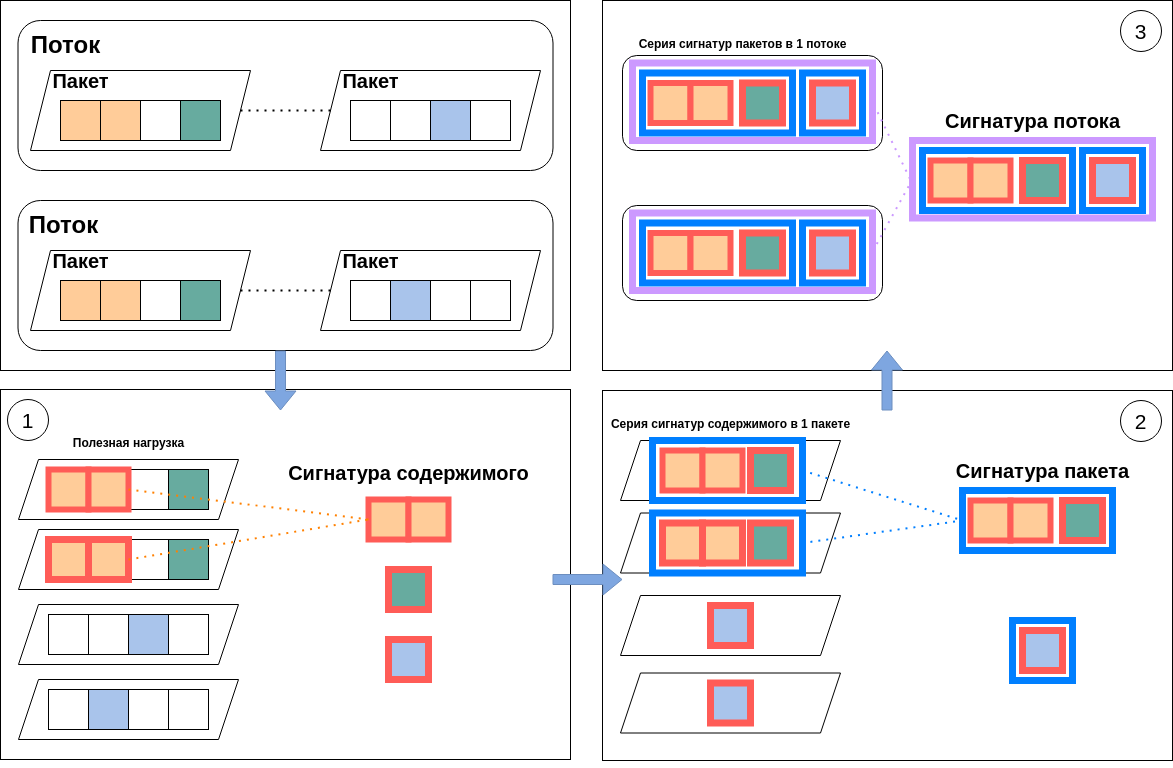
\includegraphics[width =\textwidth]{signature_structure.png}
        \caption{Процесс извлечения предлагаемой структуры сигнатур полезной нагрузки.}
    \end{center}
\end{figure}

Сигнатура содержимого определяется как различимая и уникальная подстрока полезной нагрузки, состоящая из непрерывных символов или шестнадцатеричных значений.
На самом деле уникальность с помощью одной подстроки тяжело обеспечить, например, такие строки ``GET''  или ``HTTP'', которые часто встречаются в HTTP,
не могут служить конечными сигнатурами, так как они не различают приложения.

Сигнатура пакета состоит из серии сигнатур содержимого, которые появляются в одном пакете.
Так как классификация может выполняться без накопления пакетов, т.е. без сбора потока, то анализируется всегда хотя бы один пакет.
Это значит, что для классификации не имеет смысла использовать отдельно сигнатуру содержимого.

Сигнатура потока состоит из серии сигнатур пакетов, которые появляются в одном потоке, где под потоком понимается набор пакетов, имеющий одни и те же
IP-адрес источника, IP-адрес назначения, порт источника, порт назначения и используемый протокол транспортного уровня.
Сигнатура потока гораздо более специфична для конкретного приложения, чем сигнатура пакета, и значительно повышает точность.

Заметим, что данная структура сигнатур обладает свойством вложенности.

\subsection{Метрики оценки качества сигнатур}

Для оценки качества получаемых сигнатур рассмотрим матрицу ошибок: 4 стандартные категории,
к котором можно отнести результат работы классификатора на полученной сигнатуре.
В нашем случае рассматриваемый класс это целевой протокол или приложение.
Под классификацией трафика будем понимать классификацию конкретного пакета или потока в зависимости от того, какой уровень сигнатур используется.

\begin{table}[H]
\centering
\resizebox{\columnwidth}{!}
{
    \begin{tabular}{|c|c|c|}
    \hline
                                                                                                  & Принадлежит классу (P) & Не принадлежит классу (N) \\ \hline
    \begin{tabular}[c]{@{}c@{}}Предсказана принадлежность\\ к классу (T)\end{tabular}             & TP                     & TN                        \\ \hline
    \begin{tabular}[c]{@{}c@{}}Предсказано отсутствие \\ принадлежности к классу (F)\end{tabular} & FP                     & FN                        \\ \hline
    \end{tabular}
}
\end{table}

\begin{itemize}
    \item истинно положительный (TP): указывает, что трафик правильно классифицирован, как относящийся к определенному классу.
    \item истинно отрицательный (TN): указывает, что трафик правильно классифицирован, как не относящийся к определенному классу.
    \item ложно положительный (FP): указывает, что трафик неправильно классифицирован, как относящийся к определенному классу.
    \item ложный отрицательный (FN): указывает, что трафик неправильно классифицирован, как не относящийся к определенному классу.
\end{itemize}

Наиболее часто используемые показатели для классификации трафика определяются следующим образом:

\begin{itemize}
    \item Accuracy (достоверность) - доля правильных классификаций.
    $$ accuracy = \dfrac{TP + TN}{TP + TN + FP + FN} $$

    \item Recall (полнота) - отношение верно классифицированного трафика определенному классу к общему числу трафика этого класса,
    т.е. описывает способность сигнатуры обнаружить данный целевой протокол или приложение.
    $$ recall = \dfrac{TP}{TP + FN} $$

    \item Precision (точность) - доля верно классифицированного трафика среди всего трафика, который классификатор отнёс к этому классу.
    $ precision = \cfrac{TP}{TP + FP}$

    \item $F_1$-score ($F_1$-мера) - гармоническое среднее между точностью и полнотой.
     $$ \textit{$F_1$-score} = \dfrac{2 \times recall \times precision}{recall + precision} $$
    Метрика accuracy может терять свой смысл в задачах с сильно неравными классами.
    Напротив же recall и precision не зависят от соотношения классов и поэтому применимы в случае несбалансированных классов,
    что является правдой для сетевого трафика. Часто на практике возникает задача найти оптимальный баланс между precision
    и recall. Для этих целей подходит F-мера, которая достигает максимума при recall
    и precision равным 1, и стремится к минимуму, если хотя бы один из параметров стремится к нулю.


\end{itemize}

Для сигнатур полезно ещё ввести такое понятие как:

\begin{itemize}
    \item Redundancy (избыточность) опредялется как:
    $$ \textit{Redundancy} = \frac{\text{Объём трафика идентифицированный двумя и более сигнатурами}}{\text{Объём трафика идентифицированый набором сигнатур}}$$
    Redundancy имеет значение от 0 до 1, где 0 - наилучшее значение, которое указывает на то, что все сигнатуры набора классифицируют исключительно только свою часть трафика,
    т.е. являются уникальными и незаменяемыми. Если redundancy близка к 1, то в наборе присутствует ненужные сигнатуры, которые идентифицируют перекрывающийся трафик.
    По мере увеличения количества сигнатур увеличиваются и накладные расходы системы, поэтому данное значение должно оставаться низким.
\end{itemize}

\subsection{Обзор существующих методов автоматической генерации сигнатур}

Рассмотрим несколько существующих методов автоматической генерации сигнатур и опишем основной принцип их работы.

\subsubsection{LASER}

В статье \cite{park2008towards} описан алгоритма LASER (Application Signature ExtRaction),
который основан на задаче поиска наиболее длинной общей подпоследовательности LCS (Longest common subsequence).
Данный алгоритм автоматически определяет достоверный шаблон в полезной нагрузке пакета без предварительного знания форматов протоколов, т.е. генерирует сигнатуру пакета.
За шаг извлечения сигнатуры был принят алгоритм LCS, который в основном использовался для сопоставления последовательностей ДНК в приложениях биоинформатики.
Он был модифицирован под текущие задачи.

Вводятся ограничения на модификацию LCS:

\begin{itemize}
    \item \textbf{Количество пакетов в потоке}.
    Нет необходимости проводить проверку над всеми пакетами в наборе,
    потому что сигнатура существует в нескольких начальных пакетах потока.
    \item \textbf{Минимальная длина подстроки}. Стоимость сопоставления сигнатур пропорциональна их длинам.
    Сгенерированная сигнатура состоит из последовательности подстрок.
    Чтобы избежать каких-либо тривиальных сигнатур,
    минимальная граница длины подстроки должна рассматриваться как ограничение для модифицированного алгоритма LCS.
    Имея это ограничение длины, мы предотвращаем включение однопозиционных и многопозиционных символов в последовательность общих строк,
    например символа '/' в HTTP пакетах.
    \item \textbf{Сравнение размера пакетов}. Это увеличивает вероятность нахождения надёждной сигнатуры,
    если пакеты сгруппированы по назначению (например, управляющий трафик или трафик загрузки) и характеристикам трафика.
    Одной из такой характеристик является размер пакета.
    Из графика видно, что обьём данных при установлении соединения небольшой. Конкретная сигнатура существует только в первых пакетах.
    Поэтому сравнения небольших пакетов установки соединения и пакетов загрузки нежелательно для генерации надёжной сигнатуры.

\end{itemize}

Приведём сам алгоритм из статьи:

\begin{lstlisting}[language=PL/I]
procedure Signature_Generation ()
    Flow_Pool {F1[]...Fx[]} <- Santized_packet_collector
    F1[] <- Iterate, packet dump for Flow 1
    F2[] <- Iterate, packet dump for Flow 2
    while i from 0 to packet_constraint do
        while j from 0 to packet_constraint do
            if |F1[i].packet_size - F2[j].packet_size| < threshold
            result_LCS <- LASER (F1[i], F1[j])
            LCS_Pool{} <- Append result_LCS, end if
        j++, end while
    i++, end while
    S <- select the longest from LCS_Pool
    while i from 0 to number of rest flows of Flow_Pool do
        Fi <- select one from the rest of Flow_Pool
        result_LCS <- LASER (S, Fi)
        S <- select the longest from result_LCS
    i++, end while
    return S

procedure LASER (PacketA[1...m], PacketB[1...n])
    PacketA [m...1] <- Reverse byte stream
    PacketB [n...1] <- Reverse byte stream
    Matrix [m][n]
    while i from 0 to m do
        while j from 0 to n do
            if i = 0 or j = 0, then Matrix[i][j] = 0;
            else if PacketA[i] = PacketB[j], then
                Matrix [i][j] <- 'Diagonal',
                Matrix [i][j] = Matrix [i-1][j-1] + 1;
            else if Matrix[i-1][j] >= Matrix[i][j-1], then
                Matrix[i][j] <- 'Up',
                Matrix[i][j] = Matrix [i-1][j];
            else
                Matrix[i][j] <- 'Up',
                Matrix[i][j] = Matrix [i][j-1];
        end while
    end while
    i <- m-1; j <- n-1 /* Tracking */
    while Matrix[i][j] != 0 do
        if Matrix[i][j] = 'Left', then
            j--
        else if Matrix[i][j] = 'Up', then
            i--
        else if Matrix[i][j] = 'Diagonal', then do
            Substring <- Append PacketA[i]
            if Matrix[i-1][j-1] != 'Diagonal', then
                Substring <- Append special break point character (e.g. '/')
    i--; j--, end while
    while tokenizing substring based on break point do
        if token_length > minimum_substring_length_constraint
            then, result_LCS <- Append token_substring
    end while
    return result_LCS
\end{lstlisting}

Поясним работу алгоритма. К моменту генерации сигнатуры у нас есть набор потоков,
в которых содежится хотя бы по \#\_packet\_constraint (параметр нашего алгоритма) пакетов (строка 2).
Дальше из них произвольно выбираются два потока (строки 3-4). Затем происходит полный попарный перебор пакетов из двух потоков,
и в случае, если разница размеров пакетов в паре меньше threshold (параметр нашего алгоритма),
то вызывается функция LASER для этой пары пакетов (поиск наиболее длинной общей подпоследовательности),
а результат работы заносится в пул (строки 5-11).
Из этого пула выбирается самая длинная общая подпоследовательность (строка 12).
Затем происходит процесс уточнения: проходим по всем оставшимся потокам, вызываем функцию LASER для всех пакетов из выбранного потока и текущей сигнатуры,
среди результатов выбирается самая длинная общая подпоследовательность (строки 13-17). Когда потоки в пуле закончились, возвращаем полученный результат (строка 18).

Функция LASER представляет собой алгоритм Needleman-Wunsch, в котором используется матрица направлений.
Так как пакеты развернуты (строки 21-22), то на самом деле матрица заполняется с конца (строки 23-37).
Затем обходится в обратном порядке, по направлениям и собирается общая подпоследовательность (строки 38-48).
Дальше из общей подпоследовательности, состоящая из токенов, выкидываются те, что короче minimum\_substring\_length\_constraint (параметр нашего алгоритма) (строки 49-53).
И возвращаем полученный результат (строка 50).

Таким образом, у LASER 3 параметра настройки алгоритма:
\begin{itemize}
    \item packet\_constraint (количество пакетов в потоке)
    \item threshold (порог разницы размеров для сравнения пакетов)
    \item minimum\_substring\_length\_constraint (минимальная длина подстроки)
\end{itemize}

\subsubsection{AutoSig}

Следующий рассматриваемый метод называется AutoSig \cite{santosautomatic,ye2009autosig}.

\newpage
